\documentclass[letterpaper]{article}
\usepackage[utf8]{inputenc}
\usepackage[parfill]{parskip}    % Activate to begin paragraphs with an empty line rather than an indent
\usepackage{graphicx}
\usepackage{amssymb}
\usepackage{amsmath}
\usepackage{amsthm}
\usepackage{mathtools}

\usepackage{afterpage}

\usepackage{algorithm}
\usepackage{algpseudocode}

\usepackage{verse}

\newtheorem{theorem}{Theorem}[section]
\newtheorem{corollary}{Corollary}[theorem]
\newtheorem{lemma}[theorem]{Lemma}

\theoremstyle{remark}
\newtheorem*{remark}{Remark}

\usepackage{epstopdf}
\usepackage{circuitikz}
\usepackage[separate-uncertainty = true,multi-part-units=single]{siunitx}
\usepackage{booktabs}
\usepackage{enumitem}
\usepackage[toc,page]{appendix}
\usepackage{color}
\usepackage{pgfplots}
\usepackage{pgfplotstable}
\usepackage{caption}
\usepackage{subcaption}
\usepackage{url}
\usepackage{multirow}
\usepackage{makecell}
\usepackage[round]{natbib}   % omit 'round' option if you prefer square brackets
\usepackage{titling}
\usepackage{siunitx}

\usepackage{setspace}
% \doublespacing
\usepackage{float}


\pgfplotsset{compat=1.14}

%  Special math symbols
%       floor, ceiling, angled brackets
%-----------------------------------------------------------------------
\newcommand{\floor}[1]{\left\lfloor #1\right\rfloor}
\newcommand{\ceil}[1]{\left\lceil #1\right\rceil}
\newcommand{\etal}{\textit{et al.}}
\newcommand{\RE}{\mathbb{R}}        % real space
\newcommand{\ZZ}{\mathbb{Z}}        % integers
\newcommand{\NN}{\mathbb{N}}        % natural numbers
\newcommand{\eps}{{\varepsilon}}    % prettier epsilon
%-----------------------------------------------------------------------
%  Tighter lists
%-----------------------------------------------------------------------
\newenvironment{itemize*}% Tighter itemized list
  {\begin{itemize}%
    \setlength{\itemsep}{-0.5ex}%
    \setlength{\parsep}{0pt}}%
  {\end{itemize}}
\newenvironment{description*}% Tighter description list
  {\begin{description}%
    \setlength{\itemsep}{-0.5ex}%
    \setlength{\parsep}{0pt}}%
  {\end{description}}
\newenvironment{enumerate*}% Tighter enumerated list
  {\begin{enumerate}%
    \setlength{\itemsep}{-0.5ex}%
    \setlength{\parsep}{0pt}}%
  {\end{enumerate}}
%-----------------------------------------------------------------------
% Typing shortcuts
%-----------------------------------------------------------------------
\newcommand{\X}{\mathbb{X}}
\newcommand{\SG}{\mathbf{S}}
\newcommand{\GE}{\mathcal{G}}
\newcommand{\ST}{\,:\,}
\renewcommand{\tilde}[1]{\widetilde{#1}}
\newcommand{\diam}{\mathrm{diam}}
\newcommand{\sq}{\square}
\newcommand{\half}[1]{\frac{#1}{2}}
\newcommand{\inv}[1]{\frac{1}{#1}}
\newcommand{\alg}{\textsf{SplitReduce}}
\newcommand{\sz}[1]{\sigma_{#1}}
\newcommand{\LL}{\mathcal{L}}
\newcommand{\softOmega}{\widetilde{\Omega}} 
\newcommand{\softO}{\widetilde{O}}
\newcommand{\OO}{O^*}  %or \widetilde{O}?

\newcommand{\norm}[1]{\left\lVert#1\right\rVert}

\newcommand{\dx}{\mathrm{d}x}
\newcommand{\dy}{\mathrm{d}y}
\newcommand{\dz}{\mathrm{d}z}
\newcommand{\dt}{\mathrm{d}t}
\newcommand{\du}{\mathrm{d}u}
\newcommand{\dtheta}{\mathrm{d}\theta}
\newcommand{\dq}{\mathrm{d}q}
\newcommand{\diff}{\mathrm{d}}
\newcommand{\dV}{\mathrm{d}V}
\newcommand{\dL}{\mathrm{d}L}
\newcommand{\dA}{\mathrm{d}A}
\newcommand{\dH}{\mathrm{d}H}
\newcommand{\df}{\mathrm{d}f}
\newcommand{\dg}{\mathrm{d}g}
\newcommand{\dr}{\mathrm{d}r}
\newcommand{\dw}{\mathrm{d}w}
\newcommand{\dv}{\mathrm{d}v}
\newcommand{\dI}{\mathrm{d}I}

\newcommand*\len[1]{\overline{#1}}

\DeclarePairedDelimiter\abs{\lvert}{\rvert}%

\newcommand\note[1]{\marginpar{\textcolor{red}{#1}}}
\newcommand*{\tageq}{\refstepcounter{equation}\tag{\theequation}}

\newcommand*{\equals}{=}

\usepackage{fancyhdr}

\pgfplotscreateplotcyclelist{grayscale}{
    thick,white!10!black,mark=x,mark options=solid, dashed\\%
    thick,white!20!black,mark=o,mark options=solid\\%
}

\newcommand{\mat}[1]{\ensuremath{\begin{bmatrix}#1\end{bmatrix}}}
\newcommand{\eqn}[1]{\begin{alignat*}{2}#1\end{alignat*}}
\newcommand{\p}[2]{\frac{\partial #1}{\partial #2}}
\newcommand*{\thus}{&\implies\quad&}

\newcommand{\answer}[1]{\framebox{$\displaystyle #1 $}}

 
\pagestyle{fancy}
\fancyhf{}
\rhead{Rahul Arya}
\lhead{EE 16B}
\cfoot{\thepage}

\title{Lecture 6 - Notes}
\author{Rahul Arya}
\date{February 2019}
\begin{document}

\maketitle

\section{Overview}
Using the method of phasors, we now know how to analyze the steady state of any AC circuit. We will now explore some applications of these circuits, and begin to explore techniques for designing these circuits to fit a set of requirements.

\section{Filters}
One very common use for AC circuits is as a \emph{filter}. We have seen filters before briefly, with circuits blocking either low or high frequencies. The key idea behind filters is that of \emph{superposition}. Recall, from EE16A, that in circuits consisting solely of sources and resistors, each independent source could be considered apart from the rest, with the final signal simply being the sum of all the intermediate responses from each of the sources.

Here, rather than looking at the superposition of independent sources, we will look at the superposition of input signals at the same point but with different frequencies. For notational convenience, let
\[
    G_\omega(\tilde{X}) = \frac{1}{2} \left(\tilde{X}e^{j\omega t} + \overline{\tilde{X}} e^{-j\omega t} \right).
\]
Basically, $G_w(\tilde{X})$ converts the signal with angular frequency $\omega$ represented by the phasor $\tilde{X}$ from the frequency domain to the time domain.

Specifically, we assert that if we supply some input signal of the form
\[
    V_{in}(t) = \sum_i G_{\omega_i}(\tilde{X_i})
\]
to a circuit with transfer function $H(\omega)$, the output voltage will be
\[
    V_{out}(t) = \sum_i G_{\omega_i}(H(\omega_i)\tilde{X_i}).
\]
The above is an immediate consequence of the fact that all the differential equations that describe a single-input single-output AC system are linear. Though we will not prove it formally, it should be fairly clear intuitively.

The practical consequence of the above assertion is that we can treat the superposition of signals of two different frequencies as if the two signals were separate. For instance, if we supplied an AC circuit acting as a low-pass filter with the superposition of a \SI{60}{\hertz} signal and a \SI{100}{\kilo\hertz} noise signal, the high-frequency noise would be attenuated independently of the low-frequency signal.

Now, we will consider various filter configurations, and study their behavior. For now, we will look at \emph{L filters} - filters consisting of two circuit elements placed in series, as shown:
\begin{center}
\begin{circuitikz}[european]
\draw (0, 0) to[R, l=$Z_1$] (2, 0) to[R, l=$Z_2$] (2, -2) node[ground] {};
\draw (2, 0) to (3, 0) node[ocirc] {} node[right] {$V_{out}$};
\draw (0, 0) node[ocirc] {} node[left] {$V_{in}$};
\end{circuitikz}
\end{center}

Recall from the impedance divider equation that the transfer function of this circuit is
\[
    H(\omega) = \frac{Z_2}{Z_1 + Z_2}.
\]

We will now consider all the possible forms of impedances that we can substitute into this equation. There are nine possible configurations, since we know of three different components in an AC circuit:
\begin{itemize}
    \item Both components are resistors, as shown:
    \begin{center}
    \begin{circuitikz}[american]
    \draw (0, 0) to[R, l=$R_1$] (2, 0) to[R, l=$R_2$] (2, -2) node[ground] {};
    \draw (2, 0) to (3, 0) node[ocirc] {} node[right] {$V_{out}$};
    \draw (0, 0) node[ocirc] {} node[left] {$V_{in}$};
    \end{circuitikz}
    \end{center}
    This forms a simple resistive voltage divider, which we have seen many times before, so we will not discuss it again here.
    \item Both components are inductors, as shown:
    \begin{center}
    \begin{circuitikz}[american]
    \draw (0, 0) to[L, l=$L_1$] (2, 0) to[L, l=$L_2$] (2, -2) node[ground] {};
    \draw (2, 0) to (3, 0) node[ocirc] {} node[right] {$V_{out}$};
    \draw (0, 0) node[ocirc] {} node[left] {$V_{in}$};
    \end{circuitikz}
    \end{center}
    Substituting the known form for the impedance of an inductor into our equation for the transfer function, we obtain
    \[
        H(\omega) = \frac{j\omega L_2}{j\omega L_1 + j\omega L_2} = \frac{L_2}{L_1 + L_2}.
    \]
    Thus, this circuit exhibits behavior very similar to a resistive voltage divider, with its transfer function independent of frequency. Notice, however, that unlike resistors, inductors do not dissipate energy. A natural question to ask would be: what happens to the energy if we supply a DC voltage ($\omega = 0$) to this circuit? Surely there will be some current flowing between the two potentials, which would cause energy to be dissipated, but where can this energy go? The resolution to this issue relies on the observation that our expression for $H(\omega)$ resolves to $0 / 0$ for $\omega = 0$, since our simplifications assumed that $\omega \ne 0$. In the case of $\omega = 0$, it turns out that we can no longer model the inductors as being ideal - rather, their internal resistance will have an effect of dissipating energy.
    \item Both components are capacitors, as shown:
    \begin{center}
    \begin{circuitikz}[american]
    \draw (0, 0) to[C, l=$C_1$] (2, 0) to[C, l=$C_2$] (2, -2) node[ground] {};
    \draw (2, 0) to (3, 0) node[ocirc] {} node[right] {$V_{out}$};
    \draw (0, 0) node[ocirc] {} node[left] {$V_{in}$};
    \end{circuitikz}
    \end{center}
    Substituting the known form for the impedance of a capacitor into our equation for the transfer function, we obtain
    \[
        H(\omega) = \frac{\frac{1}{j \omega C_2}}{\frac{1}{j \omega C_1} + \frac{1}{j \omega C_2}} = \frac{C_1}{C_1 + C_2}.
    \]
    Notice that here we again get something very similar to a voltage divider. Here, however, when $\omega = 0$ no current is permitted to flow, since the capacitors act as open circuits. A charge sharing argument will nevertheless demonstrate that $V_{out}$ will remain as we have claimed.
    \item One component is an inductor, and the other is a capacitor. We will discuss this circuit later, when we look at a phenomenon known as resonance.
    \item One component is a resistor, and the other is an inductor. There are two possible configurations of these two components. One of them is as follows:
    \begin{center}
    \begin{circuitikz}[american]
    \draw (0, 0) to[R, l=$R$] (2, 0) to[L, l=$L$] (2, -2) node[ground] {};
    \draw (2, 0) to (3, 0) node[ocirc] {} node[right] {$V_{out}$};
    \draw (0, 0) node[ocirc] {} node[left] {$V_{in}$};
    \end{circuitikz}
    \end{center}
    The above has the transfer function
    \[
        H(\omega) = \frac{j\omega L}{R + j\omega L} = \frac{j \omega \frac{L}{R}}{1 + j \omega \frac{L}{R}} = \frac{j\omega / \omega_p}{1 + j\omega / \omega_p},
    \]
    where $\omega_p = 1 / \tau = L/R$ is the reciprocal of the time constant $\tau$ of an LR circuit, known as the \emph{pole frequency}\footnote{Although we did not look at the transient analysis of LR circuits explicitly, the approach is very similar to that done in Lecture 2 for an RC circuit.}.
    
    The other configuration is as follows:
    \begin{center}
    \begin{circuitikz}[american]
    \draw (0, 0) to[L, l=$L$] (2, 0) to[R, l=$R$] (2, -2) node[ground] {};
    \draw (2, 0) to (3, 0) node[ocirc] {} node[right] {$V_{out}$};
    \draw (0, 0) node[ocirc] {} node[left] {$V_{in}$};
    \end{circuitikz}
    \end{center}
    The above has the transfer function
    \[
        H(\omega) = \frac{R}{R + j\omega L} = \frac{1}{1 + j \omega \frac{L}{R}} = \frac{1}{1 + j\omega / \omega_p},
    \]
    with $\omega_p$ as defined previously.
    
    \item One component is a resistor, and the other is an inductor. There are two possible configurations of these two components. One of them is as follows:
    \begin{center}
    \begin{circuitikz}[american]
    \draw (0, 0) to[R, l=$R$] (2, 0) to[C, l=$C$] (2, -2) node[ground] {};
    \draw (2, 0) to (3, 0) node[ocirc] {} node[right] {$V_{out}$};
    \draw (0, 0) node[ocirc] {} node[left] {$V_{in}$};
    \end{circuitikz}
    \end{center}
    The above has the transfer function
    \[
        H(\omega) = \frac{\frac{1}{j\omega C}}{R + \frac{1}{j\omega C}} = \frac{1}{1 + j\omega RC} = \frac{1}{1 + j\omega / \omega_p},
    \]
    where $\omega_p = 1 / \tau$ as before. This time, however, since we have an RC-circuit, $\tau = RC$. The other configuration is as follows:
    \begin{center}
    \begin{circuitikz}[american]
    \draw (0, 0) to[R, l=$R$] (2, 0) to[C, l=$C$] (2, -2) node[ground] {};
    \draw (2, 0) to (3, 0) node[ocirc] {} node[right] {$V_{out}$};
    \draw (0, 0) node[ocirc] {} node[left] {$V_{in}$};
    \end{circuitikz}
    \end{center}
    The above has the transfer function
    \[
        H(\omega) = \frac{R}{R + \frac{1}{j\omega C}} = \frac{j\omega RC}{1 + j\omega RC} = \frac{j \omega / \omega_p}{1 + j\omega / \omega_p},
    \]
    with $\omega_p$ as defined earlier.
\end{itemize}

That was a lot of filters! But looking closely at their transfer functions, excluding those filters behaving like a voltage divider, we see two distinct forms:
\eqn{
    && H(\omega) &= \frac{1}{1 + j\omega / \omega_p} \\
    && H(\omega) &= \frac{j \omega / \omega_p}{1 + j\omega / \omega_p}.
}
Since the behavior of an AC circuit is solely determined by its transfer function, understanding the above two functions will be sufficient to analyze any of the above filters (except for the LC filters, which we will discuss in a future lecture).

The first of these two transfer functions describes a \emph{low-pass filter}, since for values of $\omega \to 0$, $H(\omega) \to 1$, while for values of $\omega \to \infty$, $H(\omega) \to 0$. In essence, low frequencies can pass through, while high frequencies are sent to ground. In a symmetric manner, the second of these transfer functions describes a \emph{high-pass filter}, which has precisely the opposite behavior.

\section{Straight-line approximations}
In Lectures 4 and 6, we saw how the magnitude and phase of such transfer functions can be approximated using $2$ straight lines on a log-log plot, and provided some algebraic justification. Now, we will consider an equivalent geometric model of the situation, in order to gain further insight into why these approximations are valid.

For simplicity, we will focus on the transfer function of a low-ass filter, but the behavior for high-pass filters is analogous. Recall that any complex number can be written in polar form, so we may express $H(\omega)$ as
\eqn{
    && H(\omega) = \frac{1}{1 + j\omega / \omega_p} &= re^{j\theta} \\
    \thus 1 + j\omega / \omega_p &= \frac{1}{r} e^{-j\theta}.
}

Plotting $\frac{1}{r} e^{-j\theta} = 1 + j\omega / \omega_p$ on the complex plane for different values of $\omega$, we obtain:
\begin{center}
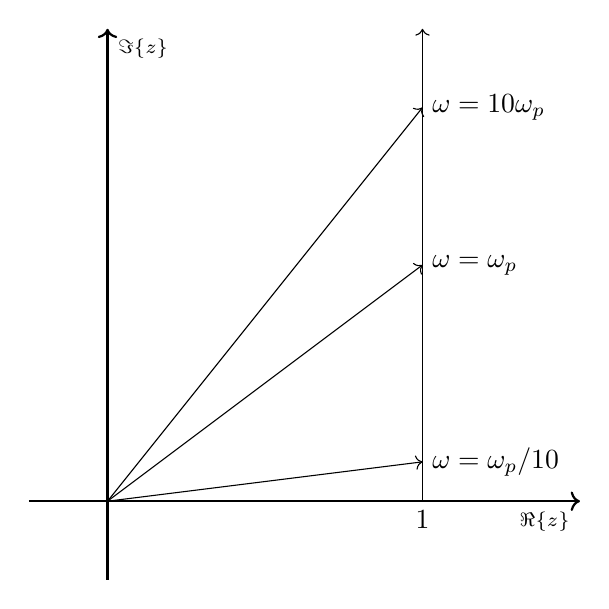
\begin{tikzpicture}
    \begin{scope}[thick,font=\scriptsize]
    \draw [->] (-1,0) -- (6,0) node [below left]  {$\Re\{z\}$};
    \draw [->] (0,-1) -- (0,6) node [below right] {$\Im\{z\}$};
    \end{scope}
    \draw [->] (0, 0) -- (4, 0.5) node[right] {$\omega = \omega_p / 10$};
    \draw [->] (0, 0) -- (4, 3) node[right] {$\omega = \omega_p$};
    \draw [->] (0, 0) -- (4, 5) node[right] {$\omega = 10\omega_p$};
    \draw [->] (4, 0) to (4, 6);
    \draw (4, 0) node[below] {$1$};
\end{tikzpicture}
\end{center}
Note that, for clarity, the above figure is not drawn to scale.

First, consider the simplest case, where $\omega = \omega_p$. Thus, from the figure (or by algebraic manipulation), we find that
\eqn{
    && \frac{1}{r} &= \sqrt{2} \\
    && -\theta &= \frac{\pi}{4}.
}

Now, imagine that the frequency of our signal is significantly below the pole frequency, with $\omega = \omega_p / 10$. Using known approximations,
\eqn{
    && \frac{1}{r} &= \left(1 + \left(\frac{1}{10}\right)^2\right)^{1/2} \\
    &&&\approx 1 + \frac{1}{2} \left(\frac{1}{10} \right)^2 \\
    &&&= 1.005 \\
    && -\theta &\approx \tan^{-1}\left(\frac{1}{10}\right) \\
    &&&\approx \frac{1}{10} \\
    &&&\approx 6^{\circ}
}

Finally, imagine that the frequency of our signal is significantly greater than the pole frequency, with $\omega = 10\omega_p$. Using known approximations,
\eqn{
    && \frac{1}{r} &= 10\left(1 + \left(\frac{1}{10}\right)^2\right)^{1/2} \\
    &&&\approx 10\left(1 + + \frac{1}{2} \left(\frac{1}{10} \right)^2 \right) \\
    &&&= 10.05 \\
    && -\theta &\approx \frac{\pi}{2} - \tan^{-1}\left(\frac{1}{10}\right) \\
    &&&\approx \frac{\pi}{4} - \frac{1}{10} \\
    &&&\approx= 90^{\circ} - 6^{\circ} \\
    &&&= 84^{\circ}.
}

Solving for our original variables $r$ and $\theta$, we obtain the values:
\begin{table}[H]
\centering
\begin{tabular}{|c|c|c|c|}
\hline
$\omega$ & $r$ & $\theta$ \\ \hline
$\omega_p / 10$ & $0.995$ & $-6^{\circ}$ \\ \hline
$\omega_p$ & $0.714$ & $-45^{\circ}$ \\ \hline
$10\omega_p$ & $0.1$ & $-84^{\circ}$ \\ \hline
\end{tabular}
\end{table}

Notice here that for very small or very large values of $\omega$, $r$ tends towards $1$ or $0$ respectively, as we already knew. However, notice also that similar behavior is true of the phase $\theta$: small values of $\omega$ lead to very little phase shift, while large values of $\omega$ induce a large phase shift. Since the goal of a low-pass filter is to let low frequencies through with a minimum of distortion, the fact that both their magnitudes and phases are preserved is very reassuring.

To approximate $r$ on a log-log scale, we simply plot the two linear approximations, as we have seen many times before. To sketch a plot of $\theta$ on a log-linear scale, however, we use three linear approximations: one at $\theta = 0$ for low frequencies, one at $\theta = -90^\circ$ for high frequencies, and a third linear approximation to model the transition between these two modes. This third approximation is drawn between the points $(\omega_p / 10, \theta(\omega = \omega_p / 10))$ and $(10\omega_p, \theta(\omega = 10\omega_p))$, as shown below:
\begin{center}
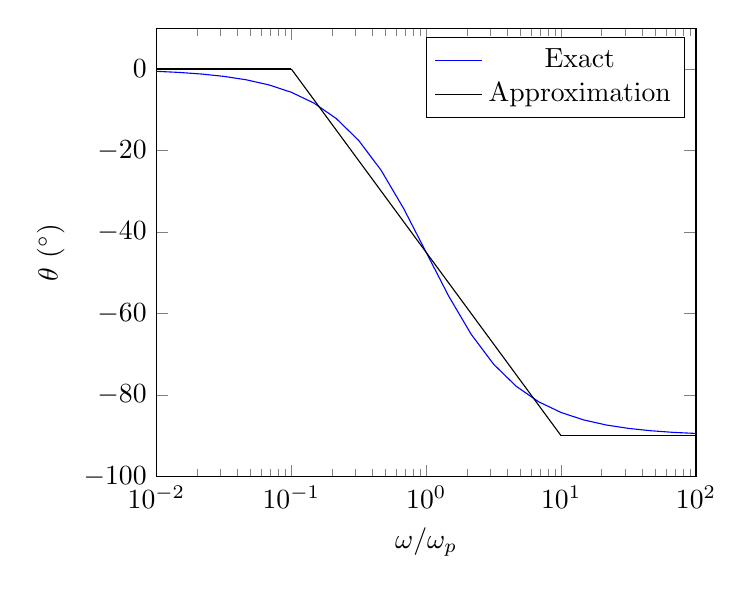
\begin{tikzpicture}
\begin{semilogxaxis}[
    xlabel=$\omega / \omega_p$, ylabel=$\theta$ (\SI{}{\degree}),
    xmin=10^(-2), xmax=10^2,
    ymin=-100, ymax=10,
    % legend style={at={(1.02,1)},anchor=north west},
 ]
\addplot [domain=0.01:100, color=blue] {(-1) * atan(x)};
\addlegendentry{Exact};
\addplot [domain=0.01:0.1] {0};
\addplot [domain=10:100] {-90};
\addplot [domain=0.1:10] {-45 * log10(x / 0.1)};
\addlegendentry{Approximation};
\end{semilogxaxis}
\end{tikzpicture}
\end{center}
Notice that this plot is least accurate near $w_p / 10$ and $10w_p$, but gets increasingly accurate as $w_p$ moves further in both extremes. Interestingly, it is also exact at $w_p$, which should have been clear from reasons of symmetry.

Of course, similar results can all be obtained for high-pass filters.

\section{Design}
Now that we have a solid understanding of low- and high-pass filters, it's time to look at a toy example. Imagine that we have a signal with amplitude \SI{1}{\milli\volt} and frequency approximately $\SI{1}{\kilo\hertz}$, as shown:
\begin{center}
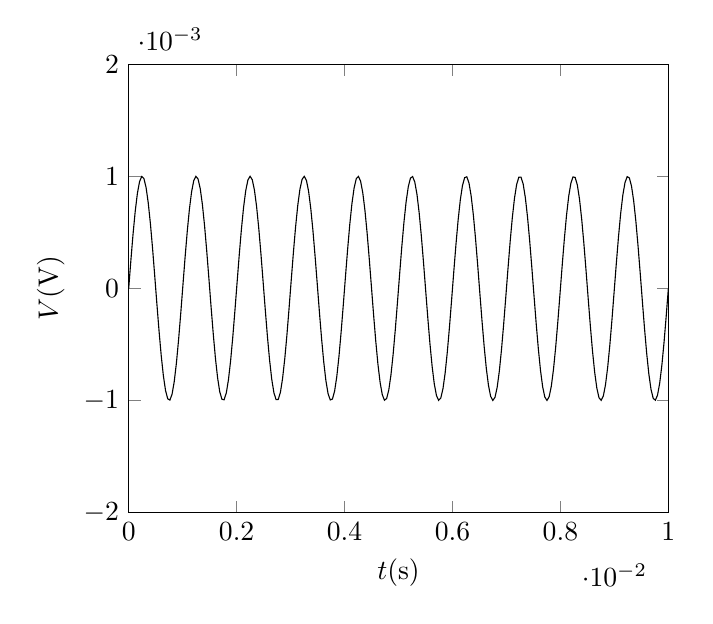
\begin{tikzpicture}
\begin{axis}[
    xlabel=$t (\SI{}{\second})$, ylabel=$V (\SI{}{\volt})$,
    xmin=0, xmax=0.01,
    ymin=-2*10^(-3), ymax=2*10^(-3),
    % legend style={at={(1.02,1)},anchor=north west},
 ]
\addplot [domain=0:0.01, samples=250] {0.001 * sin(360 * 1000 * x)};
\end{axis}
\end{tikzpicture}
\end{center}

Now, we introduce some \SI{60}{\hertz} noise (perhaps from the mains power) at \SI{20}{\milli\volt}, as well as some \SI{100}{\kilo\hertz} (perhaps from a malfunctioning fluorescent light ballast) noise at \SI{50}{\milli\volt}, which are shown superimposed on our signal below:
\begin{center}
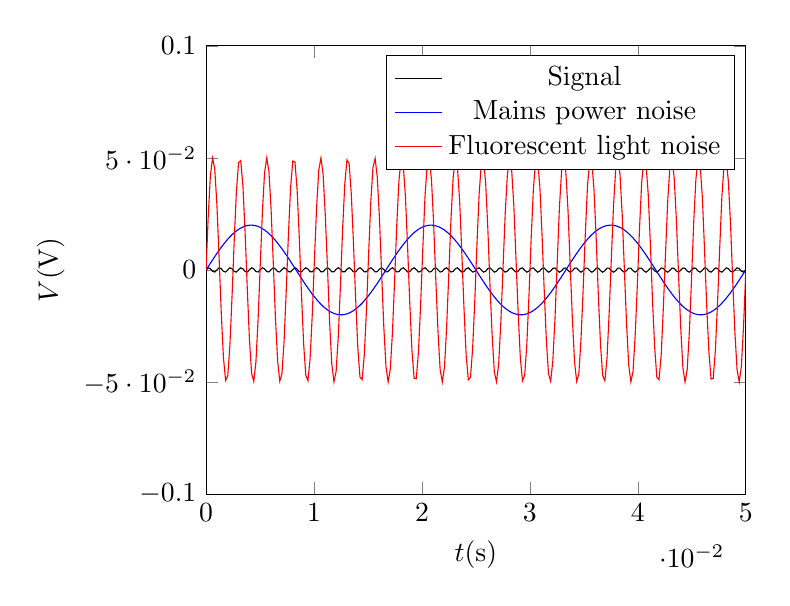
\begin{tikzpicture}
\begin{axis}[
    xlabel=$t (\SI{}{\second})$, ylabel=$V (\SI{}{\volt})$,
    xmin=0, xmax=0.05,
    ymin=-10^(-1), ymax=10^(-1),
    % legend style={at={(1.02,1)},anchor=north west},
 ]
\addplot [domain=0:0.05, samples=250] {0.001 * sin(360 * 1000 * x)};
\addlegendentry{Signal}
\addplot [domain=0:0.05, samples=250, color=blue] {0.020 * sin(360 * 60 * x)};
\addlegendentry{Mains power noise}
\addplot [domain=0:0.05, samples=250, color=red] {0.050 * sin(360 * 100000 * x)};
\addlegendentry{Fluorescent light noise}
\end{axis}
\end{tikzpicture}
\end{center}
Adding these noise sources to our signal, we obtain the resultant signal
\begin{center}
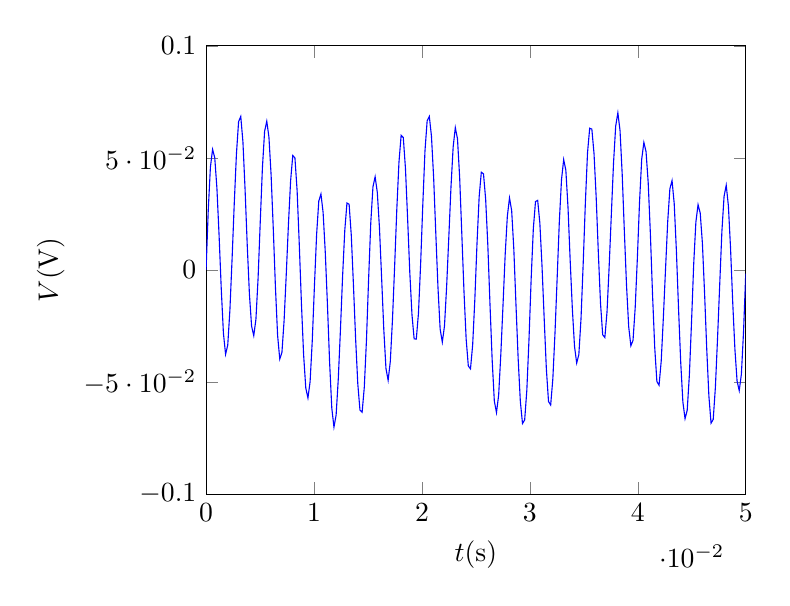
\begin{tikzpicture}
\begin{axis}[
    xlabel=$t (\SI{}{\second})$, ylabel=$V (\SI{}{\volt})$,
    xmin=0, xmax=0.05,
    ymin=-10^(-1), ymax=10^(-1),
    % legend style={at={(1.02,1)},anchor=north west},
 ]
\addplot [domain=0:0.05, samples=250, color=blue] {0.001 * sin(360 * 1000 * x) + 0.020 * sin(360 * 60 * x) + 0.050 * sin(360 * 100000 * x)};
\end{axis}
\end{tikzpicture}
\end{center}
At this point, our original signal is not even visible!

However, this is the 21st century! You may have heard of the Fourier transform, which can break up a signal into its constituent sinusoids. All we need to do is record this signal precisely in a digital format, send it to a computer, and let a CS major figure the rest out.

Unfortunately, we are encoding this signal using a $4$-bit ADC, much like the one from lab. Recall that our ADC had a maximum voltage of \SI{3.3}{\volt}, and had a least significant bit (in other words, a precision) of
\[
    \frac{\SI{3.3}{\volt}}{2^4} \approx \SI{0.2}{\volt}.
\]
But our signal only has an amplitude \SI{1}{\milli\volt}! What to do?

The natural response is to amplify our signal, perhaps using an op-amp circuit from EE16A, until the amplitude of our signal is of the same order as our measurement ability. To do so, we will need to amplify by a factor of at least
\[
    \frac{\SI{3.3}{\volt}}{\SI{1}{\milli\volt}} = 3300.
\]
Unfortunately, when we do this, our noise signals will shoot up, reaching amplitudes of
\[
    \SI{50}{\milli\volt} \cdot 3300 = \SI{165}{\volt}!
\]
Of course, our op-amps can only produce voltages between their rails, which we might set to $\pm \SI{5}{\volt}$. So our amplified signal will rail much of the time. Plotting the end result of this amplification, we obtain:
\begin{center}
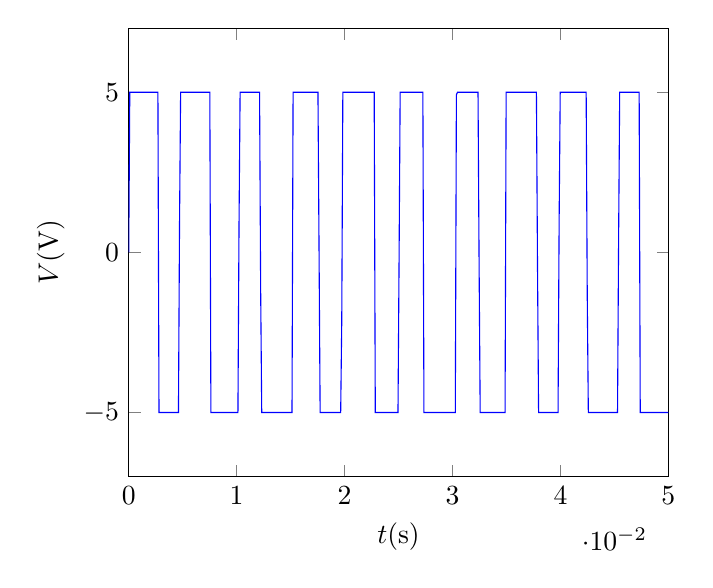
\begin{tikzpicture}
\begin{axis}[
    xlabel=$t (\SI{}{\second})$, ylabel=$V (\SI{}{\volt})$,
    xmin=0, xmax=0.05,
    ymin=-7, ymax=7,
    % legend style={at={(1.02,1)},anchor=north west},
 ]
\addplot [domain=0:0.05, samples=500, color=blue] {min(max(3300 * (0.001 * sin(360 * 1000 * x) + 0.020 * sin(360 * 60 * x) + 0.050 * sin(360 * 100000 * x)), -5), 5)};
\end{axis}
\end{tikzpicture}
\end{center}
Notice that our signal has railed for a significant portion of the cycle, meaning that information has been irretrievably lost before ever getting to a computer.

Clearly, analog processing is necessary in order to remove the noise from our circuit.
\end{document}
